% TEX TS-program = xelatex
% !TEX encoding = UTF-8 Unicode
% Inbuilt themes in beamer
\documentclass{beamer}
\usepackage{amsmath, amsfonts, amssymb, amsthm}
\usepackage{graphicx}
% \usepackage{ifpdf,mla}
\usepackage{fontspec}
\usepackage{ulem}
\usepackage{booktabs}
\usepackage{caption} 
\usepackage{subfigure}
\usepackage{theorem}
\usepackage{xeCJK}
\usepackage{setspace}
\usepackage{multirow}
\usepackage{booktabs}
\usepackage{subfigure}
\usepackage{eurosym}
\usepackage{textcomp}
\usepackage{romannum}
\usepackage{multirow}
\usepackage{verbatim}
\usepackage{float}
\usepackage{rotfloat}
\usepackage{array}
\newcolumntype{C}[1]{>{\centering\let\arraybackslash}p{#1}}

% Theme/Font choice:
\usetheme{Berkeley}
\usecolortheme{dolphin}
\usefonttheme{serif}
\setbeamerfont{title}{series=\bfseries}
% \setbeamerfont{frametitle}{size=\huge}
\setmainfont{Minion Pro}
\setCJKmainfont{宋體-繁}
\setbeamertemplate{footline}[frame number]
\beamertemplatenavigationsymbolsempty %removing navigation symbols
\setbeamertemplate{enumerate item}{\alph{enumi}.}
% \renewcommand{\baselinestretch}{1.2}
% \setmainfont{Times New Roman}
% \setsansfont{宋體-繁}

% Title page details: 
\title[]{The Impact of Tariffs on Price and Welfare: Literature Reviews and Future Research Plans}
\author[]{Ming-Chieh, Chang}
\institute{National Taiwan University}
\date{\today}

\begin{document}

% Title page frame
\begin{frame}
    \titlepage 
\end{frame}

\begin{frame}{Outline}
    \tableofcontents
\end{frame}

\section{Introduction}
\begin{frame}{Introduction}
    \underline{\textbf{Trade Economics}}
    \begin{itemize}
        \item Price effects
        \item Welfare effects
        \item Distributional effects
        \item Productivity effects
    \end{itemize}

    \vspace{3mm}

    \underline{\textbf{US-China Trade War}}
    \begin{itemize}
        \item Started 2018
        \item Literatures: econometric methods and quantitative models
        \item Affected {\color{red}Taiwan} since we are highly {\color{red}export-oriented}
    \end{itemize}
\end{frame}


\section{Price and Basic Welfare Impact}
\begin{frame}{Price and Basic Welfare Impact}
    \underline{\textbf{When Export Supply Is {\color{red}Not} Perfectly Elastic}}
    \begin{figure}[H]
        \centering
        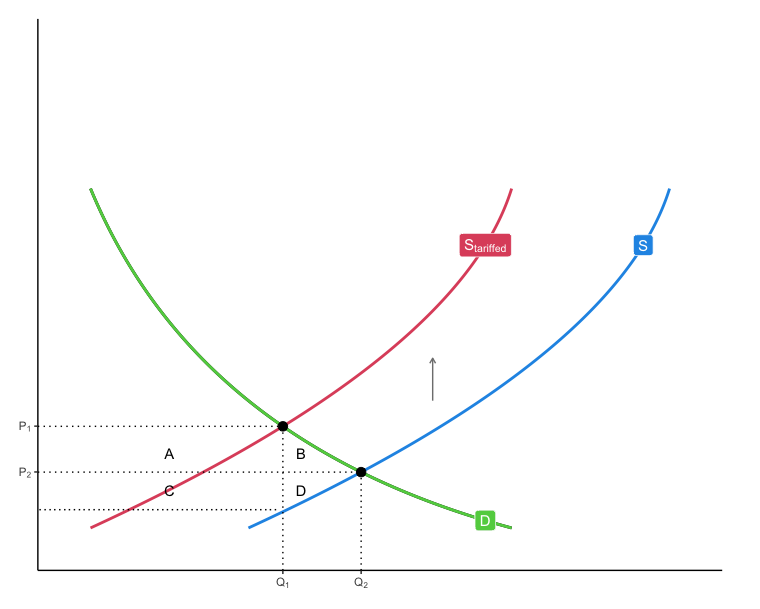
\includegraphics[width=0.55\textwidth]{tariff_welfare.png}
    \end{figure}
    \begin{itemize}
        \item Consumer price {\color{red}rises,} producer price recieved {\color{red}falls}
        \item Consumer's tax burden is rectangle A
        \item {\color{red}Producer also bear tax burden C}
    \end{itemize}
\end{frame}

\begin{frame}{Price and Basic Welfare Impact}
    \underline{\textbf{When Export Supply {\color{red}Is Perfectly Elastic}}}
    \begin{figure}[H]
        \centering
        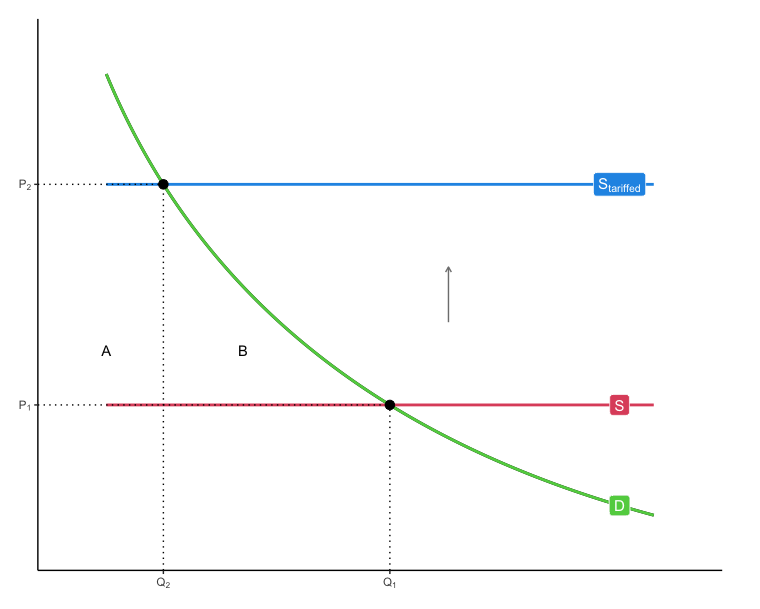
\includegraphics[width=0.55\textwidth]{Tariff_welfare_flat.png}
    \end{figure}
    \begin{itemize}
        \item Consumer price {\color{red}rises more,} producer price recieved {\color{red}unchanged}
        \item Consumer's tax burden is a {\color{red}bigger} rectangle A
        \item {\color{red}Producer bears no tax burden}
    \end{itemize}
\end{frame}

\begin{frame}{Price and Basic Welfare Impact}
    \underline{\textbf{Empirics in the US-China Trade War}}
    \begin{itemize}
        \item Amiti et al. (2019), Fajgelbaum et al. (2020), and many other papers: 
        almost {\color{red}perfectly elastic} export supply
        \item Improting consumers bear all burdens 
        \item {\color{red}"complete pass-through"} of import tariffs to consumers
    \end{itemize}
\end{frame}

\section{Distributional Effects and Rationales of the Trade War}
\begin{frame}{Distributional Effects \\ and Rationales of the Trade War}
\underline{\textbf{Distributional Effects}}
\begin{itemize}
    \item Winners: producers
    \begin{itemize}
        \item Exporters did {\color{red}not} pay tariff since tariffs were paid by foreign consumers
        \item {\color{red}Domestic price rose} since imported goods were tariffed
    \end{itemize}
    \item Losers: consumers: paid tariffs
    \begin{itemize}
        \item Counties in the Midwestern Plains were hit hardest by retaliatory tariffs
    \end{itemize}
\end{itemize}
\end{frame}

\begin{frame}{Distributional Effects \\ and Rationales of the Trade War}
\underline{\textbf{Rationales of the Trade War: {\color{red}Political} perspectives}}
\begin{itemize}
    \item 2016 presidential election data combined
    \item Fajgelbaum et al. (2020): {\color{red}Politically competitive} counties were protected the most by US tariffs
    \item Consistent to the logic of {\color{red}majority voting}
    \item Relatively suggestive
\end{itemize}
\end{frame}

\section{Productivity Effects from Tariffs}
\begin{frame}{Productivity Effects from Tariffs}
\underline{\textbf{{\color{red}"Within"} An Industry}}
\begin{itemize}
    \item Melitz (2003): in a heterogeneous firm trade model, firms with {\color{red}higher productivity}
    \begin{itemize}
        \item expand to larger scale
        \item gain more market share
        \item increase market efficiency
    \end{itemize}
    \item Tariffs may {\color{red}block} productivity growth
\end{itemize}
\end{frame}

\begin{frame}{Productivity Effects from Tariffs}
\underline{\textbf{{\color{red}"Between"} industries}}
\begin{itemize}
    \item Krugman (1987): {\color{red}learning-by-doing} model
    \begin{itemize}
        \item Firms {\color{red}cumulate} experience and {\color{red}improve productivity} by time
        \item Temporary government protections keep infant industries from stringent foreign competitions
    \end{itemize}
    \item Tariffs {\color{red}help} productivity accumulation
\end{itemize}
\end{frame}

\begin{frame}{Productivity Effects from Tariffs}
    \underline{\textbf{{Discussions}}}
    \begin{itemize}
        \item No contradiction in the above two model
        \item {\color{red}"Within"} or {\color{red}"between"} industries matters
        \item Productivity is hard to measure
        \item Literature in the US-China trade war in this remained small
    \end{itemize}
\end{frame}

\section{Effects of the US-China Trade War on Taiwan}
\begin{frame}{Effects of the US-China Trade War on Taiwan}
\underline{\textbf{Why does the US-China Trade War matter to Taiwan?}}
\begin{itemize}
    \item Taiwanese firms are largely {\color{red}export-oriented}, especially toward the US and China
    \item US high tariffs to Chinese goods may be {\color{red}good for Taiwanese exportes in the short run}
    \item {\color{red}Loss of purchasing power globally} may hurt them in the long run
    \item We do not know which channels are the most influential, so {\color{red}econometric estimations} are needed
\end{itemize}
\end{frame}

\begin{frame}{Effects of the US-China Trade War on Taiwan}
    \underline{\textbf{Future Research Plan}}
    \begin{itemize}
        \item Estimate the gain of exporters in the short run
        \item Conncet trade policy making with {\color{red}political} considerations
        \item Evaluate trade policy, give suggestions based on empirical evedence
        \item Productivity estimations are extensions
    \end{itemize}
\end{frame}

\end{document}